\chapter{Symulacja dynamiczna}\label{chap:dynamic}

\section{Założenia i konfiguracja}

Eksperymenty dynamiczne wykonano w tym samym środowisku obliczeniowym co testy statyczne. Każda symulacja obejmuje 30 kroków, a po każdej mutacji sieci algorytmy otrzymują maksymalnie 45~s na ponowne zbilansowanie licencji. Analizowano dwie konfiguracje licencyjne -- Duolingo Super oraz dominowanie rzymskie. Do testów wykorzystano różne typy grafów: losowe, bezskalowe oraz małoświatowe.

Testy przeprowadzono dla sześciu profili mutacji: trzech syntetycznych, które charakteryzują się prostą logiką modyfikacji (low, med, high), oraz trzech bardziej złożonych i realistycznych, które uwzględniają mechanizmy takie jak preferencyjne przyłączanie, domykanie triad czy losowe przekształcanie krawędzi (pref\_triadic, pref\_pref, rand\_rewire).

Warianty \emph{low}, \emph{med} oraz \emph{high} różnią się prawdopodobieństwami modyfikacji wierzchołków i krawędzi (tabela~\ref{tab:dyn-mutation-levels}).

\begin{table}[H]
  \centering
  \caption{Parametry intensywności mutacji w symulacji dynamicznej.}
  \label{tab:dyn-mutation-levels}
  \begin{tabular}{lcccc}
    \toprule
    \textbf{Poziom} & \textbf{Dodawanie węzłów} & \textbf{Usuwanie węzłów} & \textbf{Dodawanie krawędzi} & \textbf{Usuwanie krawędzi} \\
    \midrule
    low             & 0.02                      & 0.01                     & 0.06                        & 0.04                       \\
    mid             & 0.06                      & 0.04                     & 0.18                        & 0.12                       \\
    high            & 0.12                      & 0.08                     & 0.30                        & 0.20                       \\
  \end{tabular}
\end{table}


Dodatkowo zbadano trzy bardziej realistyczne profile ewolucji sieci. Wszystkie operują na tych samych limitach liczby dodawanych/usuwanych elementów co warianty syntetyczne, różnią się jednak mechanizmem wyboru sąsiedztwa.

Wariant \emph{pref\_triadic} łączy dwa mechanizmy typowe dla sieci społecznych: preferencyjne przyłączanie i domykanie triad. Nowe węzły dołączają do sieci, preferencyjnie łącząc się z istniejącymi węzłami o wysokim stopniu (zasada "bogaci stają się bogatsi"). Nowe krawędzie powstają natomiast poprzez domykanie trójkątów -- wyszukiwanie dwóch niepołączonych węzłów, które mają wspólnego sąsiada, i tworzenie między nimi połączenia. Mechanizm ten wzmacnia lokalną strukturę klastrową sieci, co odzwierciedla tendencję do tworzenia zamkniętych grup w rzeczywistych sieciach.

Wariant \emph{pref\_pref} stosuje mechanizm preferencyjnego przyłączania zarówno przy dodawaniu nowych węzłów, jak i tworzeniu krawędzi między już istniejącymi. Oznacza to, że nie tylko nowe węzły chętniej łączą się z popularnymi wierzchołkami, ale również nowe krawędzie z większym prawdopodobieństwem powstaną między dwoma węzłami, które już teraz mają wysoki stopień. Takie podejście intensywnie promuje tworzenie centralnych hubów w sieci, co jest kluczową cechą topologii bezskalowych.

Wreszcie wariant \emph{rand\_rewire} wprowadza do sieci element losowości, inspirowany modelem Wattsa--Strogatza. Nowe węzły dołączane są w sposób losowy, bez preferencji dla popularniejszych wierzchołków. Zamiast dodawania nowych krawędzi, model ten modyfikuje istniejącą strukturę poprzez operację "przełączania" (rewiring): losowa krawędź jest usuwana, a jeden z jej końców jest następnie łączony z innym, losowo wybranym węzłem w sieci. Proces ten prowadzi do powstawania "skrótów" i zmniejsza regularność struktury grafu.


\section{Algorytm zachłanny}

W tym wariancie algorytm zachłanny w każdym kroku symulacji buduje rozwiązanie całkowicie od zera. Stanowi to dolną granicę narzutu czasowego dla metod bez pamięci oraz bazowy punkt odniesienia jakości, do którego porównujemy bardziej zaawansowane metaheurystyki korzystające z rozwiązań z poprzedniego kroku.

\subsection{Zestawienie dla wszystkich mutacji}
Tabela~\ref{tab:greedy-cold-summary} zestawia średni koszt na węzeł i średni czas na krok dla sześciu badanych profili mutacji: trzech syntetycznych oraz trzech realistycznych. Wszystkie czasy mieszczą się w przedziale 0.5--1.8 ms na krok, a średni koszt na węzeł oscyluje wokół 0.46--0.48.

\begin{table}[H]
  \centering
  \caption{Algorytm zachłanny: średni koszt na węzeł oraz średni czas na krok dla wszystkich wariantów mutacji.}
  \label{tab:greedy-cold-summary}
  \begin{tabular}{lcc}
    \toprule
    \textbf{Metoda mutacji} & \textbf{Koszt/węzeł (mean)} & \textbf{Średni czas [s]} \\
    \midrule
    high                    & 0.48009                     & 0.00159                  \\
    low                     & 0.47983                     & 0.00165                  \\
    med                     & 0.47491                     & 0.00181                  \\
    pref\_pref              & 0.46371                     & 0.00083                  \\
    pref\_triadic           & 0.46787                     & 0.00053                  \\
    rand\_rewire            & 0.47556                     & 0.00083                  \\
    \bottomrule
  \end{tabular}
\end{table}

Algorytm zachłanny jest bardzo szybki, co potwierdza jego przydatność jako czasowy punkt odniesienia w środowisku dynamicznym. Warianty realistyczne sprzyjają nieco niższym kosztom: \texttt{pref\_pref} osiąga najniższy średni koszt (0.464), a \texttt{pref\_triadic} jest jednocześnie najszybszy (\SI{0.00053}{\s}). Wariant \texttt{rand\_rewire} jest trudniejszy (0.476), ale pozostaje bardzo szybki czasowo.

Różnice kosztu dla mutacji syntetycznych są niewielkie (0.475--0.480), natomiast czasy są wyższe niż w profilach realistycznych, szczególnie dla \texttt{med/high}. Wskazuje to, że bardziej lokalne, realistyczne przekształcenia struktury grafu są łatwiejsze do obsłużenia. Czasy dla \texttt{pref\_pref} wynoszą średnio \SI{0.00083}{\s}, a dla \texttt{pref\_triadic} \SI{0.00053}{\s}, co potwierdza ich przewagę czasową nad mutacjami syntetycznymi (\SI{0.00159}{\s} dla \texttt{high}).

\section{Analiza mutacji syntetycznych}
\subsection{Metaheurystyki}

Tabela~\ref{tab:dyn-synth-warm} przedstawia zbiorcze wyniki dla różnych metod mutacji. Średni koszt na węzeł jest bardzo zbliżony dla wszystkich poziomów intensywności, z jedynie nieznacznym wzrostem dla wariantu \texttt{high}. Sugeruje to, że algorytmy są w stanie skutecznie adaptować się do zmian w topologii sieci.

Średni czas wykonania algorytmu rośnie wraz z intensywnością mutacji. Wariant \texttt{low} jest najszybszy, podczas gdy \texttt{high} wymaga najwięcej czasu na ponowne zbilansowanie. Jest to naturalna konsekwencja faktu, że większa liczba modyfikacji grafu (dodawanie/usuwanie węzłów i krawędzi) stanowi większe wyzwanie obliczeniowe dla algorytmów optymalizacyjnych. Mimo to, różnice w czasach nie są drastyczne, co świadczy o dobrej skalowalności zastosowanych metod.

\begin{table}[H]
  \centering
  \caption{Wyniki dla różnych metod mutacji.}
  \label{tab:dyn-synth-warm}
  \begin{tabular}{lcc}
    \toprule
    \textbf{Metoda mutacji} & \textbf{Średni koszt} & \textbf{Średni czas [s]} \\
    \midrule
    high                    & 0.4893                & 3.169                    \\
    med                     & 0.4850                & 3.075                    \\
    low                     & 0.4852                & 2.878                    \\
    \bottomrule
  \end{tabular}
\end{table}

\subsection{Profil kosztu i czasu w czasie}
Jako przykład ewolucji kosztu i czasu w krokach symulacji wybrano algorytm genetyczny. Rysunki~\ref{fig:dyn-synth-genetic-cost} i~\ref{fig:dyn-synth-genetic-time} przedstawiają odpowiednio przebieg kosztu na węzeł oraz czasu wykonania w zależności od kroku symulacji dla różnych poziomów intensywności mutacji.

Dla wariantu \texttt{high} można zaobserwować niewielkie, lecz zauważalne wahania średniego kosztu na węzeł, które nie są tak widoczne w przypadku wariantów \texttt{low} i \texttt{med}. Jeśli chodzi o czasy wykonania, dla każdego z trzech wariantów widoczne są zbliżone wahania w trakcie trwania symulacji.

\begin{figure}[H]
  \centering
  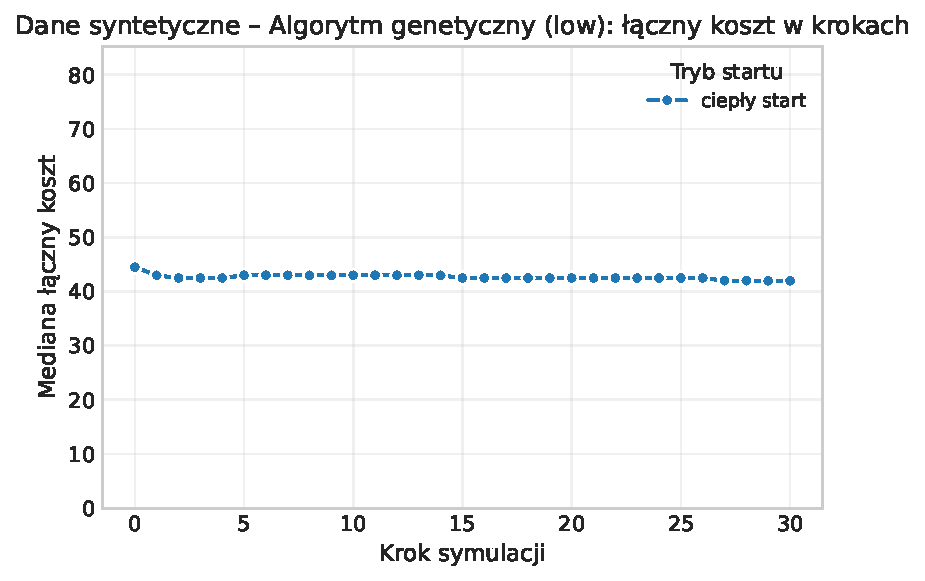
\includegraphics[width=0.32\linewidth]{assets/figures/dynamic/synthetic/synthetic_algorytm_genetyczny_cost_over_steps_low.pdf}
  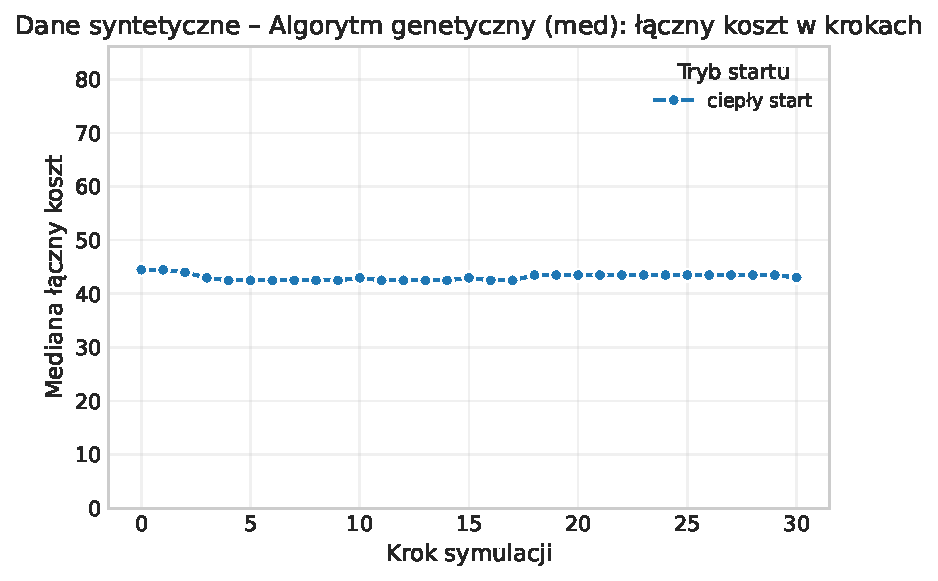
\includegraphics[width=0.32\linewidth]{assets/figures/dynamic/synthetic/synthetic_algorytm_genetyczny_cost_over_steps_med.pdf}
  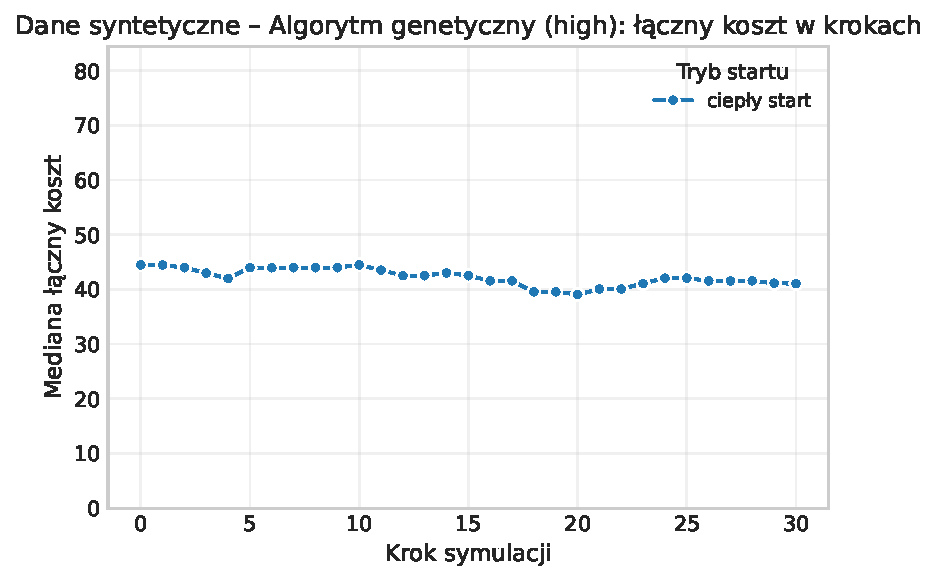
\includegraphics[width=0.32\linewidth]{assets/figures/dynamic/synthetic/synthetic_algorytm_genetyczny_cost_over_steps_high.pdf}
  \caption{Algorytm genetyczny -- koszt na węzeł w kolejnych krokach symulacji (warianty low/med/high).}
  \label{fig:dyn-synth-genetic-cost}
\end{figure}

\begin{figure}[H]
  \centering
  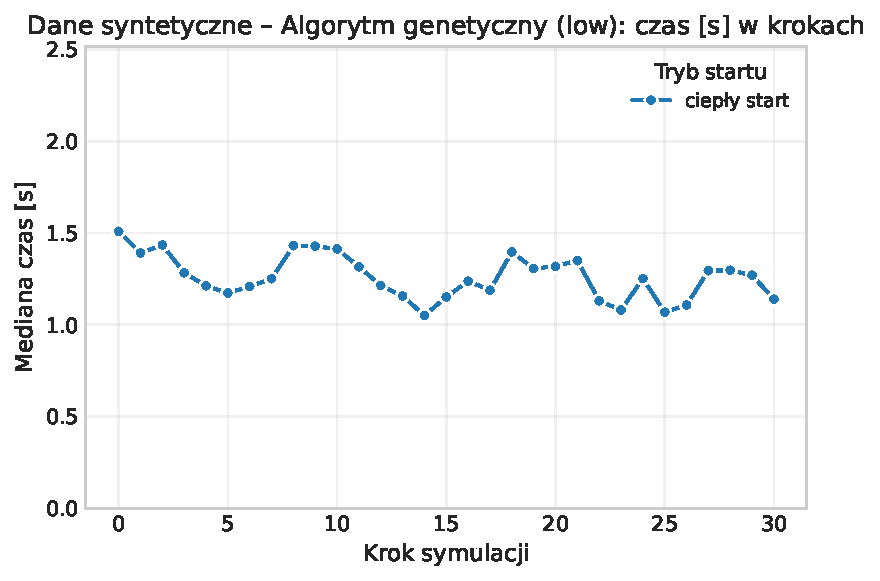
\includegraphics[width=0.32\linewidth]{assets/figures/dynamic/synthetic/synthetic_algorytm_genetyczny_time_over_steps_low.pdf}
  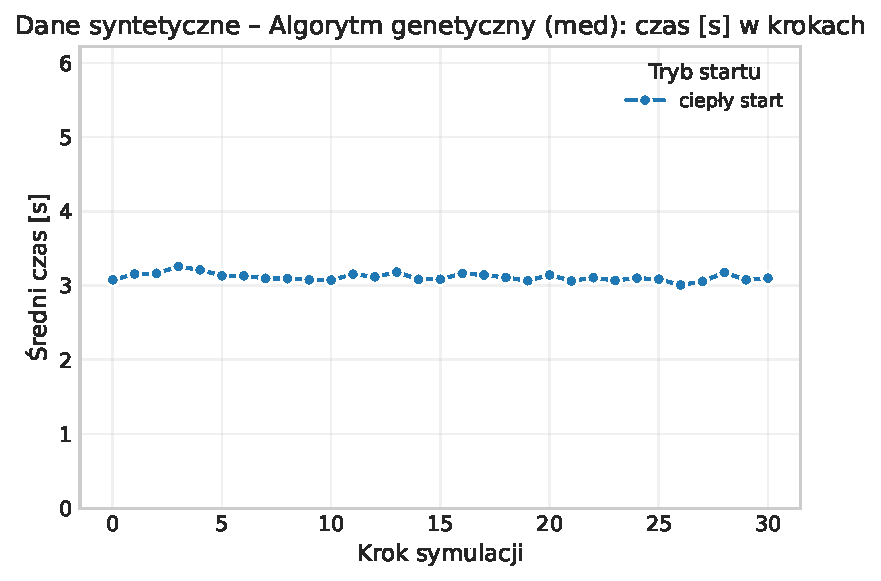
\includegraphics[width=0.32\linewidth]{assets/figures/dynamic/synthetic/synthetic_algorytm_genetyczny_time_over_steps_med.pdf}
  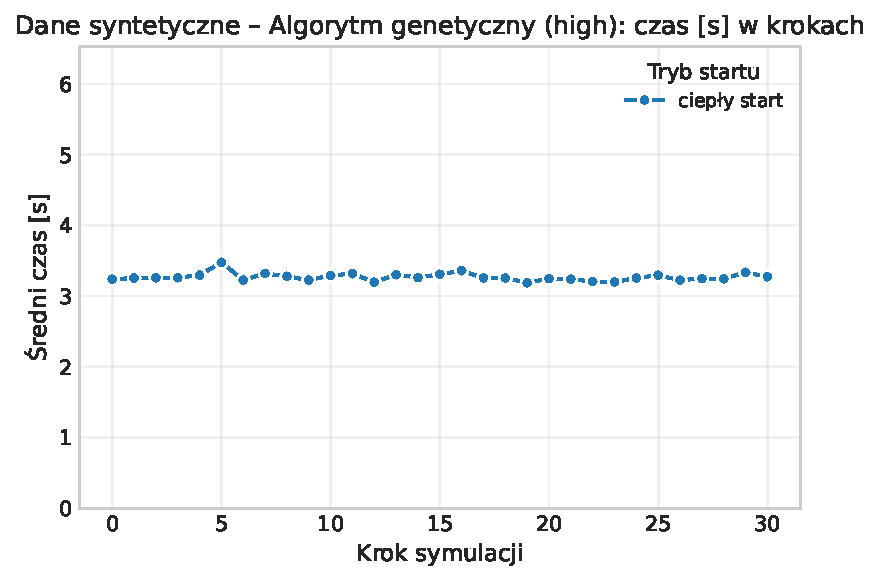
\includegraphics[width=0.32\linewidth]{assets/figures/dynamic/synthetic/synthetic_algorytm_genetyczny_time_over_steps_high.pdf}
  \caption{Algorytm genetyczny -- czas wykonania w kolejnych krokach symulacji (warianty low/med/high).}
  \label{fig:dyn-synth-genetic-time}
\end{figure}

\section{Analiza mutacji realistycznych}
Tabela~\ref{tab:dyn-real-warm} przedstawia zbiorcze wyniki dla scenariuszy realistycznych. Wariant \texttt{pref\_triadic} wyróżnia się najkrótszym średnim czasem wykonania (poniżej 1 sekundy), przy zachowaniu kosztu na poziomie zbliżonym do wariantu \texttt{pref\_pref}. Z kolei scenariusz \texttt{rand\_rewire} okazał się najbardziej wymagający dla algorytmów -- charakteryzuje się jednocześnie najwyższym średnim kosztem i najdłuższym czasem przetwarzania. Wynika to z faktu, że losowe przełączanie krawędzi zaburza lokalną strukturę klastrową sieci, zwiększa entropię topologii i utrudnia wykorzystanie poprzedniego rozwiązania jako punktu odniesienia. W efekcie optymalizacja wymaga więcej iteracji, a uzyskana jakość jest gorsza.


\begin{table}[H]
  \centering
  \caption{Wyniki dla różnych metod mutacji w scenariuszach realistycznych.}
  \label{tab:dyn-real-warm}
  \begin{tabular}{lccc}
    \toprule
    \textbf{Metoda mutacji} & \textbf{Średni koszt całkowity} & \textbf{Koszt/węzeł (mean)} & \textbf{Średni czas [s]} \\
    \midrule
    pref\_pref              & 113.34                          & 0.4764                      & 1.6774                   \\
    pref\_triadic           & 70.08                           & 0.4764                      & 0.8619                   \\
    rand\_rewire            & 116.83                          & 0.4917                      & 1.8421                   \\
    \bottomrule
  \end{tabular}
\end{table}

\subsection{Wybrane algorytmy i metody mutacji}
Poniżej wybrano kilka par algorytmów i metod mutacji, które pokazują różne kompromisy. Dla porównania uwzględniono również dwie mutacje syntetyczne. Nie są to zawsze najlepsze jakościowo konfiguracje, ale dobrze ilustrują różne scenariusze.

\begin{table}[H]
  \centering
  \caption{Wybrane pary algorytmów i metod mutacji (różne kompromisy).}
  \label{tab:dyn-synth-selected-best}
  \begin{tabular}{llccc}
    \toprule
    \textbf{Algorytm}     & \textbf{Metoda} & \textbf{Liczba kroków} & \textbf{Koszt/węzeł} & \textbf{Śr. czas [s]} \\
    \midrule
    Solver ILP            & pref\_triadic   & 434                    & 0.362                & 1.525                 \\
    Solver ILP            & rand\_rewire    & 496                    & 0.390                & 2.553                 \\
    Algorytm genetyczny   & pref\_triadic   & 744                    & 0.409                & 0.615                 \\
    Algorytm genetyczny   & pref\_pref      & 930                    & 0.414                & 1.134                 \\
    Przeszukiwanie tabu   & pref\_triadic   & 744                    & 0.413                & 1.470                 \\
    Przeszukiwanie tabu   & rand\_rewire    & 930                    & 0.445                & 2.581                 \\
    Algorytm mrówkowy     & pref\_pref      & 899                    & 0.417                & 6.906                 \\
    Algorytm mrówkowy     & pref\_triadic   & 744                    & 0.424                & 3.002                 \\
    Wyżarzanie symulowane & pref\_triadic   & 744                    & 0.460                & 0.555                 \\
    Algorytm zachłanny    & pref\_pref      & 930                    & 0.464                & 0.001                 \\
    Zbiór dominujący      & pref\_triadic   & 744                    & 0.457                & 0.005                 \\
    Algorytm losowy       & pref\_pref      & 930                    & 0.754                & 0.001                 \\
    \bottomrule
  \end{tabular}
\end{table}

Solver ILP osiąga najniższe koszty, ale wymaga około 1.5--2.6 sekundy na krok. Algorytm genetyczny dobrze sprawdza się przy zmianach klastrowych (\texttt{pref\_triadic}), oferując niski koszt i czas około 0.6 sekundy. Przy wariancie \texttt{pref\_pref} jest wolniejszy (1.1 s), ale zachowuje dobrą jakość. Z kolei wyżarzanie symulowane jest szybkie (około pół sekundy) i stabilne, ale jakościowo ustępuje bardziej zaawansowanym metodom.

Przeszukiwanie tabu korzysta z lokalności zmian, osiągając sensowny koszt i czas około 1.5 sekundy przy \texttt{pref\_triadic}. Jednak przy mutacjach losowych (\texttt{rand\_rewire}) czas wzrasta do około 2.6 sekundy, a koszt również rośnie. Algorytm mrówkowy zapewnia bardzo dobrą jakość przy \texttt{pref\_pref}, ale działa najwolniej (prawie 7 sekund). Przejście na \texttt{pref\_triadic} ponad dwukrotnie przyspiesza jego działanie kosztem niewielkiego pogorszenia jakości.

Heurystyki szybkie, takie jak algorytm zachłanny (około 1 ms) i zbiór dominujący (około 5 ms), są bardzo efektywne. Zbiór dominujący zwykle osiąga niższy koszt niż zachłanny, co czyni go dobrym wyborem przy ograniczeniach czasowych. Mutacje klastrowe (\texttt{pref\_triadic}, \texttt{pref\_pref}) pomagają wszystkim algorytmom utrzymać niski średni koszt licencji liczony na jeden węzeł i krótszy czas. Natomiast \texttt{rand\_rewire} zwiększa zarówno koszt, jak i czas.


\subsection{Ewolucja kosztów w czasie}
Pełne przebiegi dla algorytmu genetycznego pokazano na rys.~\ref{fig:dyn-real-genetic-cost}--\ref{fig:dyn-real-genetic-time}. Łączenie preferencyjnego przyłączania z triadycznym domykaniem sprzyja utrzymaniu najniższych kosztów, natomiast wariant z losowym przełączaniem krawędzi prowadzi do wolniejszej stabilizacji. Analizując koszt na węzeł na rys. \ref{fig:dyn-real-genetic-cost}, można zauważyć, że dla każdego z typów mutacji przebiega on podobnie, oscylując wokół zbliżonego poziomu.

Z kolei, patrząc na czas wykonania na rys. \ref{fig:dyn-real-genetic-time}, widać, że dla wariantu \texttt{rand\_rewire} występują największe wahania, co sugeruje większą niestabilność w procesie optymalizacji. Warianty \texttt{pref\_triadic} i \texttt{pref\_pref} charakteryzują się bardziej stabilnym czasem wykonania.

\begin{figure}[H]
  \centering
  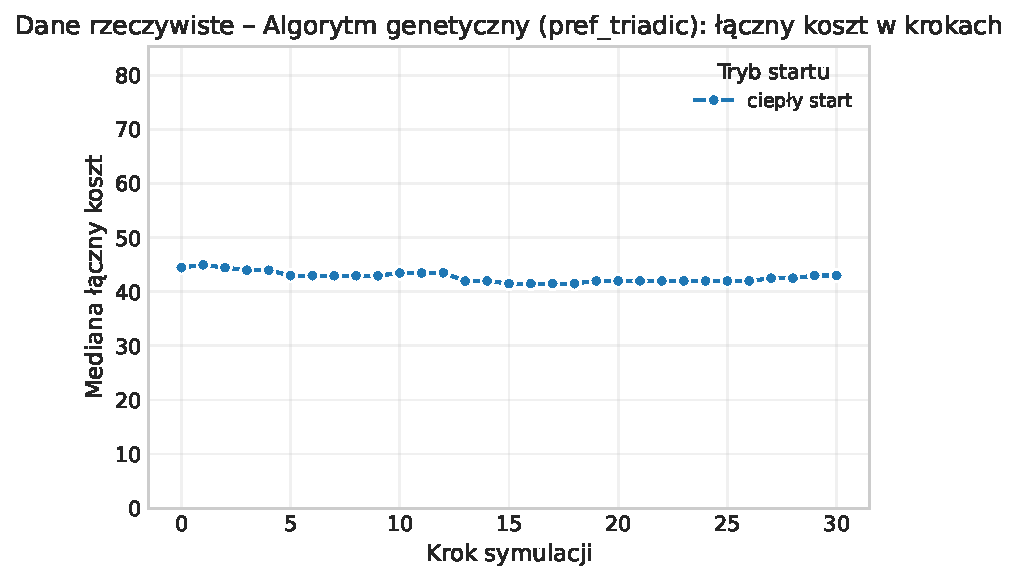
\includegraphics[width=0.32\linewidth]{assets/figures/dynamic/real/real_algorytm_genetyczny_cost_over_steps_pref_triadic.pdf}
  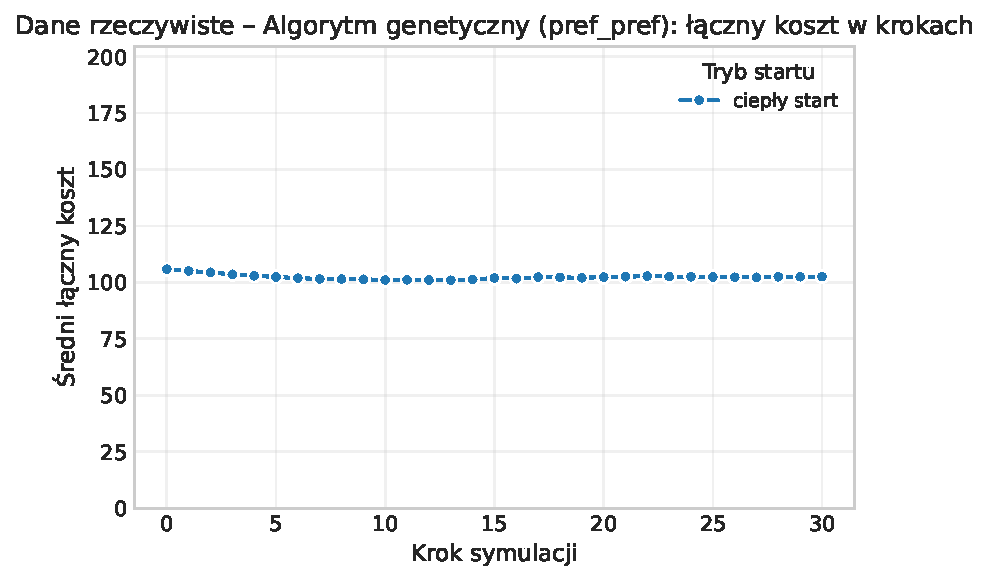
\includegraphics[width=0.32\linewidth]{assets/figures/dynamic/real/real_algorytm_genetyczny_cost_over_steps_pref_pref.pdf}
  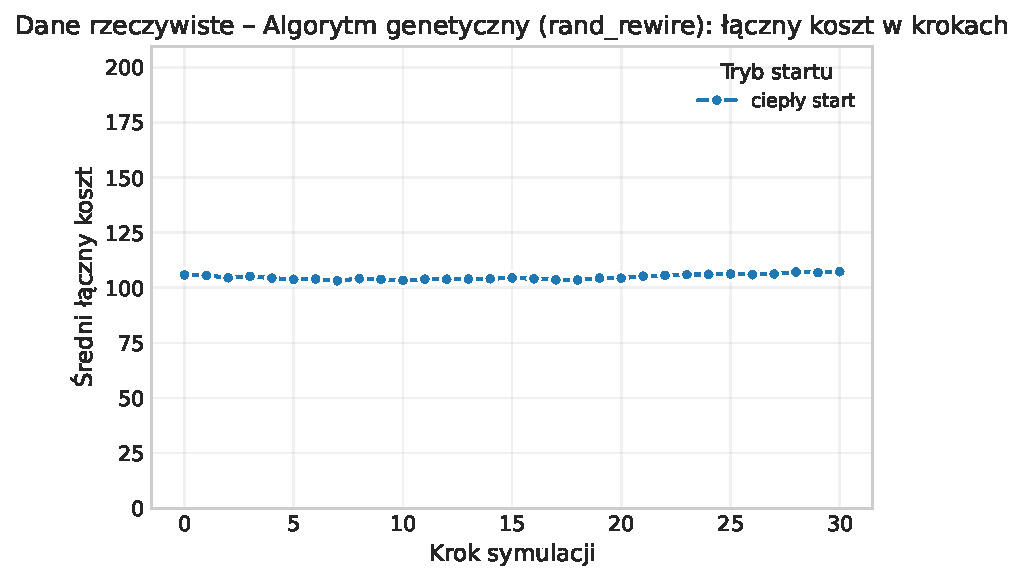
\includegraphics[width=0.32\linewidth]{assets/figures/dynamic/real/real_algorytm_genetyczny_cost_over_steps_rand_rewire.pdf}
  \caption{Algorytm genetyczny -- koszt na węzeł w wariantach realistycznych.}
  \label{fig:dyn-real-genetic-cost}
\end{figure}

\begin{figure}[H]
  \centering
  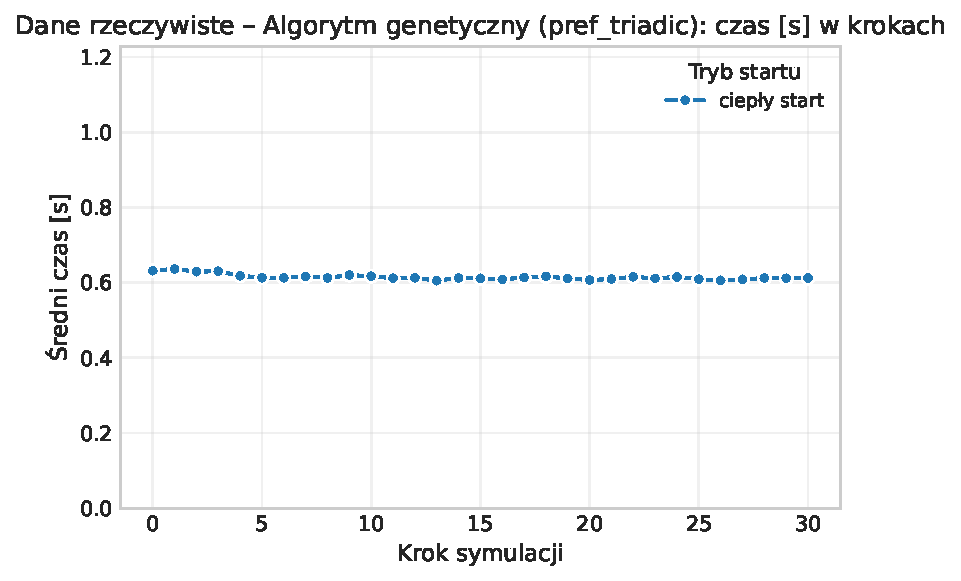
\includegraphics[width=0.32\linewidth]{assets/figures/dynamic/real/real_algorytm_genetyczny_time_over_steps_pref_triadic.pdf}
  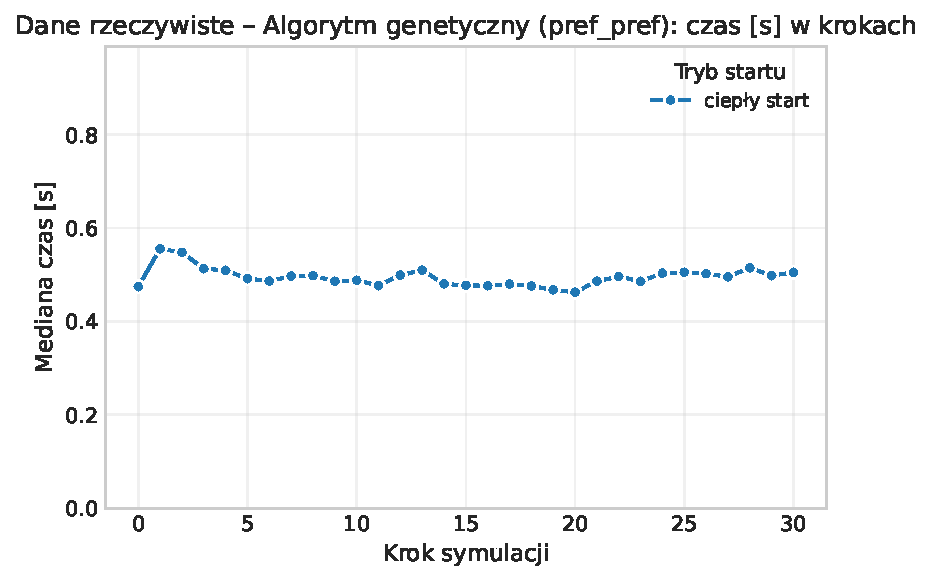
\includegraphics[width=0.32\linewidth]{assets/figures/dynamic/real/real_algorytm_genetyczny_time_over_steps_pref_pref.pdf}
  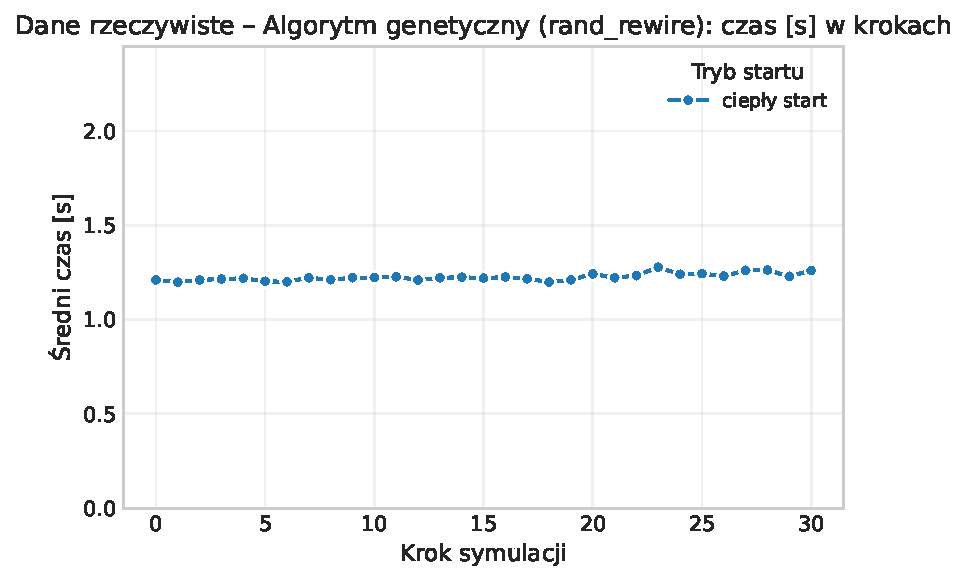
\includegraphics[width=0.32\linewidth]{assets/figures/dynamic/real/real_algorytm_genetyczny_time_over_steps_rand_rewire.pdf}
  \caption{Algorytm genetyczny -- czas wykonania w wariantach realistycznych.}
  \label{fig:dyn-real-genetic-time}
\end{figure}

\subsection{Wnioski}
Przeprowadzona analiza dynamiczna wykazała, że dobór algorytmu optymalizacyjnego w środowisku dynamicznym powinien uwzględniać zarówno profil zmian topologii sieci, jak i dostępny budżet czasowy. Badania obejmujące sześć wariantów mutacji (trzy syntetyczne oraz trzy realistyczne) na różnych typach grafów pozwoliły na sformułowanie kluczowych wniosków dotyczących adaptacji algorytmów do ewoluujących struktur sieciowych.

Mutacje realistyczne, takie jak \texttt{pref\_triadic} oraz \texttt{pref\_pref}, okazały się łatwiejsze do obsłużenia w porównaniu z wariantami syntetycznymi o wysokiej intensywności. Mechanizmy preferencyjnego przyłączania oraz domykania trójkątów sprzyjają wzmacnianiu klastrowości i tworzeniu hubów, co zmniejsza efektywny rozmiar problemu pokrycia. W rezultacie algorytmy osiągały niższe koszty (0.470--0.475 w porównaniu do 0.485--0.489) oraz krótsze czasy wykonania (0.9--1.7 s w porównaniu do 2.9--3.2 s). Z kolei mutacje typu \texttt{rand\_rewire} zwiększały entropię topologii poprzez zrywanie lokalnych połączeń, co prowadziło do najgorszych wyników zarówno pod względem kosztu (0.486), jak i czasu (1.9 s).

Algorytmy wykazywały różną odporność na poszczególne typy zmian w zależności od mechanizmu wykorzystania poprzedniego rozwiązania. Solver ILP zapewniał najwyższą jakość (koszt 0.362--0.390), lecz wymagał znacznego czasu na ponowne rozwiązanie zmodyfikowanych ograniczeń. Algorytm genetyczny dobrze radził sobie przy zmianach klastrowych, oferując korzystny kompromis między jakością a czasem (koszt 0.409 przy czasie 0.615 s dla \texttt{pref\_triadic}), jednak jego efektywność spadała w przypadku mutacji destrukcyjnych. Przeszukiwanie tabu, jako metoda intensywnie lokalna, sprawdzało się przy zmianach o ograniczonym zasięgu, lecz przy mutacjach o większej skali wymagało rozszerzenia promienia poszukiwań, co wydłużało czas działania nawet do 6.5 sekundy.

Szybkie heurystyki, takie jak algorytm zachłanny oraz zbiór dominujący, zachowywały swoją użyteczność również w środowisku dynamicznym, oferując czasy wykonania poniżej 5 ms przy kosztach porównywalnych z bardziej złożonymi metodami. Algorytm zachłanny osiągał stabilny czas w zakresie 0.5--1.8 ms przy koszcie 0.464--0.480, natomiast zbiór dominujący zapewniał nieco niższy koszt przy czasie około 5 ms.

Wyniki badań wskazują na konieczność adaptacyjnego doboru strategii optymalizacyjnej w zależności od obserwowanego profilu zmian. Przy zmianach o charakterze klastrowym zaleca się stosowanie metaheurystyk z mechanizmami naprawy poprzedniego rozwiązania. W przypadku zmian chaotycznych konieczne może być głębsze odświeżenie rozwiązania lub zaakceptowanie wyższego kosztu w zamian za stabilność czasową. W sytuacjach, w których czas stanowi krytyczne ograniczenie, szybkie heurystyki stanowią bezpieczny wybór, zapewniając przewidywalną wydajność niezależnie od typu mutacji.

Najlepszy kompromis globalny oferują metaheurystyki z mechanizmami konstrukcji opartymi na poprzednich wynikach oraz lokalnych naprawach, które można dynamicznie dostosowywać do intensywności zaobserwowanych zmian między krokami symulacji.
